\section{Problem Definition and Algorithm}

\subsection{Data set and Preprocessing}

The data used for training and test of the proposed classifier are retrieved from the Alzheimer's Disease Neuroimaging Initiative (ADNI) database. After filtering, images of 33 AD subjects and 50 NC subjects,  are downloaded. With most of these subjects are scanned more than once, we have 89 AD examples and 139 NC examples in the data set.The data set are divided into training data, test data, and validation data with a ratio of 7:2:1.

The preprocess can be divided into 4 phases (\cite{suk16}) :
	\begin{enumerate}
	\item Preprocessing of anatomical images
	\item  Preprocessing of functional images
	\item Anatomical standardization of functional images
	\item Removal of noise signa
	\end{enumerate}

The results of the preproces are a set of mean time series 
\begin{center}
$ F^{(n)} \in \{ \emph{F} | \emph{F} = \left[ \textbf{f}_1, \cdots, \textbf{f}_t, \cdots, \textbf{f}_T \right],  \textbf{f}_t \in  \mathbb{R}^{R} \}, n=1,  \cdots, N$ ,
\end{center}
where $N=228$ is number of the scans, $R=120$ is the number of  ROIs, and $T=135$ is the length of a time series. 

\subsection{Dimension Reduction with DAE}

\begin{figure}[H!]
    \centering
    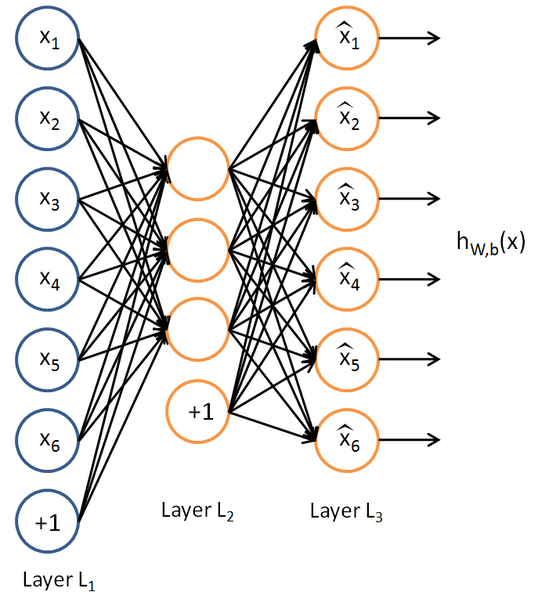
\includegraphics[width=0.9\textwidth]{autoencoder.png}
    \caption{Autoencoder}
    \label{fig:awesome_image}
\end{figure}
\begin{figure}[H!]
    \centering
    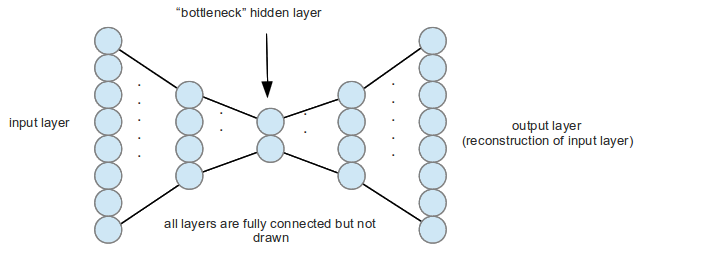
\includegraphics[width=0.9\textwidth]{stackedDAE.png}
    \caption{Stacked Autoencoder}
    \label{fig:awesome_image}
\end{figure}

\textcite{suk16} proposed that a stacked DAE can used as an intermediate building block for deeper models in neuroimaging analysis. DAE is an unsupervised multilayer feed-forward neural networks, the goal of which is setting a latent representation of feature vectors of its input by training a nonlinear approximation function $h(\textbf{f}_t) \approx \textbf{f}_t$ (Figure 1). Concretely, 
\begin{center}
$\emph{G} = \left[ \textbf{g}_1, \cdots, \textbf{g}_t, \cdots, \textbf{g}_T \right], \textbf{g}_t \in \mathbb{R}^{R}$ 
\end{center}
is expected to converted from its original form 
\begin{center}
$\emph{F} = \left[ \textbf{f}_1, \cdots, \textbf{f}_t, \cdots, \textbf{f}_T \right], \textbf{f}_t \in \mathbb{R}^{R}. $
\end{center} 

A stacked autoencoder (Figure 2) is composed of multiple layers of autoencoders, in which the outputs of each layer is fed as the inputs of successive layer \cite{stackedDAE}. Usually greedy layer-wise training is applied to train a stacked autoencoder. In current implementation, training for the stacked model is similar to the non-stacked one. Lleast-square loss function with  is selected to train the stacked model, in which the difference is directly computed between input layer and final target layer. Although that setting of the hidden layer configure is  heuristic, the combination in \textcite{suk16}'s paper is followed. 

After training, only the first part of the DAE (i.e. from input layer to bottleneck hidden layer) is used to transform each $\textbf{f}_t \in  \mathbb{R}^{R}$ into $ \textbf{x}_t \in  \mathbb{R}^{r}$, where $ r < R$. As a result, the encoded representation of a scan becomes
\begin{center}
$\emph{X} = \left[ \textbf{x}_1, \cdots, \textbf{x}_t, \cdots, \textbf{x}_T \right].$ 
\end{center}

\subsection{High-level RNN classifiers and their ensemble for subject diagnosis}

\textcite{wee15} proposes a framework for brain functional connectivity analysis, in which the time series of a scan are decomposed into multiple overlapping sub-series by a sliding window. Justified by their work, a encoded time-series is splitted into identical-sized sub-series
\begin{center}
$\emph{X} = \left[ \textbf{x}_1, \cdots, \textbf{x}_s, \cdots, \textbf{x}_{S} \right]$, where $T=n*S, n$ is an integer. 
\end{center}

A RNN is a specialized class of neural network that is suitable for dynamic temporal sequences. Connections between units in a RNN form a directed cycle. For each unit, hidden nodes are created as internal memory to process sequences of inputs, which enables RNN to condition the model on all previous units in a sequence (Figure 3). Below are the formulas in the network.

\begin{center}
$S_k = \sigma(W^{(rec)}S_{k-1} + W^{x}x_k )$
\end{center} 
\begin{center}
$y = softmax(W^{(s)}S_k)$
\end{center}

The detailed notations are explained below:
\begin{easylist}
\ListProperties(Hide=100, Hang=true, Progressive=3ex, Style*=-- )
@ $ \textbf{x}_k \in  \mathbb{R}^{r}, k=1, \cdots , n$: the input of a unit
@ $S_k $: current hidden state
@ $W^{(rec)}$: weights matrix used to condition the hidden state of the previous time-step 
@ $W^{x}$: weights matrix used to condition the input of a unit $ \textbf{x}_k$
@ $\sigma()$: the non-linearty function ()
@ $y$: predicted class for the sequence
@ $W^{(s)}$: weight matrix that transform $S_k$ to $y$
\end{easylist}

\begin{figure}[!htbp]
    \centering
    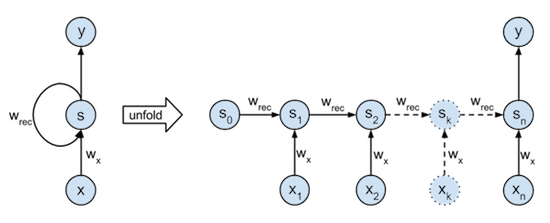
\includegraphics[width=0.9\textwidth]{rnn.png}
    \caption{Recurrent Neural Networks}
    \label{fig:awesome_image}
\end{figure}

In terms of the sub-series setting, data in each time point of a series $\textbf{x}_t$ become the input of a unit. The final output at the end of the sequence is the predicted class (AD or NC) for the whole sub-series. For the purpose of diagnosis of a subject, ensemble learning is used to predict the class for the time-series of a scan. Each high-level classifier votes with equal weight and the class with the most votes is selected as the class of a time series.
